\section{Structure}
Over all there are four components: User interface, system interface, function component, and model component.
Note however that the system interface is only used in our \nameref{sub:altSystemComponent} in subsection \ref{sub:altSystemComponent}.
This section describes how these components internal structure is.
A subsection for each component is presented below.

\subsection{User Interface Component}
This component consists of three sub-components: \cinterface[], \sinterface[], and \ainterface[].
Each of these interfaces is described in the sub-subsections bellow.

The sub-components share a login class, which is a window where a user enters his/her user name and password.
Depending on the role of the user who is logging in, he/she is directed to the main window of the corresponding interface.

Every window in the sub-components will inherit from a class called ``HelpdeskWindow''.
This class is described in paragraph \ref{par:helpdeskwindow}.\fixme{Dette er en reference til der hvor beskrivelsen af HelpdeskWindow kommer til at v\ae re. Inds\ae t gerne :)}

This entire component depends on the function component to gain any functionality. The Authenticator makes sure that a user is directed to the correct Main Window after login, the Problem Handler provides problem search, modifiability, and addition for interfaces, the \ainterface[] relies mainly on the Administrator sub-component for administrating person and departments.

\subsubsection{\cinterface[]}
The structure of the \cinterface[] is shown in figure \ref{fig:client_interface}.
Each window represents a class and the navigation arrows indicates an association between the classes.
Each object of the different classes will hold a pointer to the object(window) that created it, so it is possible to go back from one window to another.

As mentioned, each window class inherits from the HelpdeskWindow class.
Further the Client Problem View inherits from an abstract Problem View class. The reason for this is that there are different problem views -- two in the \sinterface[] -- and making one class that the others inherits from will make the views similar and thereby making the system more comprehensible for the end user.

\subsubsection{\sinterface[]}
The structure of the \sinterface[] is visualized in figure \ref{fig:Navigation_DiagramStaff}.
The windows in the figure represents classes of this component, the navigation arrows are translated to associations in UML.
Like the \cinterface[], the classes in this component



Notice that Staff Main Window aggregates the clients Main Window. Likewise does the Add Solution aggregate the Search Window from the Client sub-component.
If a staff member is an administrator he/she is presented with an administrate button in the main window, which will transfer the user to the Admin Main Window, which is described in the following sub-subsection.


\subsubsection{\ainterface[]}
Figure \ref{fig:Navigation_DiagramAdmin} shows the navigation diagram of the \ainterface[].
Every window inherits from the abstract HelpdeskWindow class.



Like the Staff Main Window aggregated the clients Main Window, the Admin Main Window aggregates the staff Main Window, thereby giving the \ainterface[] all the possibilities that the two other interfaces has.

\subsection{System Interface Component}
\fixme{Det her kan nok g�res mere udf�rligt, men ved ikke om det er meningen}
This component is responsible for connecting our system to another systems database, so that our system can use the user names, which already exists in the organization where out system is being implemented.
There is no internal structure in this component since it only has a single class which holds the responsibility fr this entire component.

This component is however connected to the Authenticator sub-component in the function component.
The connection between these components is that this component is a supplier of data for the Authenticator component.
The Authenticator component asks this component to retrieve information about a user in the database and this component provides this information if it is available.

\subsection{Function Component}
The function components main purpose is to provide functionality for the users of the system.\fixme{N\o{}dvendigt?}
This component id divided into three sub-components; Problem Handler, Administrator, and Authenticator.
These are described independently in the following sub-subsections.

\subsubsection{Problem Handler}
This sub-component is responsible for handling problems -- as the name implies.
This component consists of only a single class, which yields no internal structure.
It is though connected to the Model component, where the systems data resides.
The Problem Handler is able to operate on the model, particularly on the Problem class, but also on the Client class, Staff class, and Solution class.

The Problem Handler component can both create, modify, and delete problems as well as assigning problems to staff members.
Note however that the Problem Handler does not assign problems by it self, but rather provide the functionality for the \sinterface[].
The Solution class is handled in the sense that solutions can be attached and detached to/from problems through this component.

Both the Staff and Client classes are handle through the relations which are between these classes and the Problem class, namely Assignment, Subscription, and Comment. See subsection \ref{sub:modelComponent} for information on Assignment, Subscription, and Comment.\fixme{Skal tag ogs� skrives p� eller ligger det implicit?}

\subsubsection{Administrator}
In short this sub-component handles everything in the model which the Problem Handler does not.
This include adding, modifying, and deleting Person objects, Departments, Categories and Tags.
As well as assigning Roles to the Persons.

Like the Problem Handler, this sub-component does not do anything by it self, it simply provides functionality for the \ainterface[].

\subsubsection{Authenticator}
The Authenticator makes sure that a user is authenticated and can only commit actions appropriate for his or her Role.
This sub-component is either connected to an external database through the Login System Interface component or is connected to our systems database through our Model component.

\subsection{Model Component}
\label{sub:modelComponent}
The classes of the Model component are described in section \ref{cap:classesevents}.
However during revision of our class diagram, we decided to insert more classes.
Figure \ref{fig:modelComponent} shows our revised Model component.

\begin{figure}[hb]
	\centering
		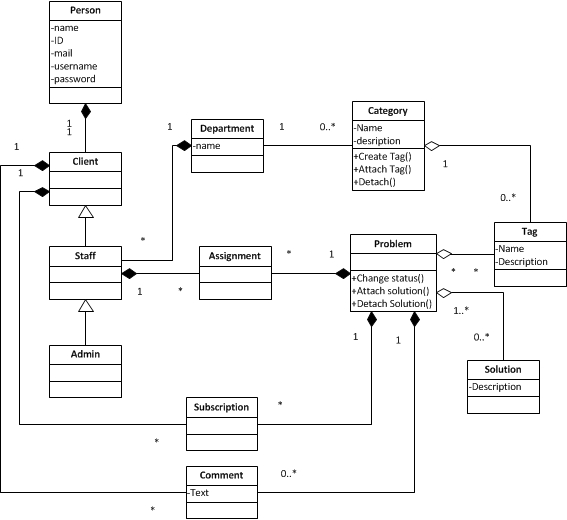
\includegraphics[width=0.80\textwidth]{input/component_design/Modelkomponent.jpg}
	\morscaption{The revised Model component}
	\label{fig:modelComponent}
\end{figure}

The new classes are: Assignment, Subscription, Comment, Tag, Category and Admin.
The two first are simply mediators between Staff and Problem, and Client and Problem respectively.
They are there to ``remember'' the events Problem Assigned and Client Subscribe.\fixme{Den findes ikke endnu, men den skal vel laves, no?}
Comment simply holds a comment for a given problem, and remembers the poster of the Comment in for of the aggregation from client.
The Tag class objects can be tied to a problem in order to ``Categorize'' it.
The Tags also belongs to a Category which again belongs to a single Department.
This way a Problem with some given Tags, can easily be sent to a Staff member of the Department which the problem is categorized to be in.\fixme{Lidt kryptisk m\aa ske..}